\documentclass[10pt, notumble, letterpaper]{leaflet}

\usepackage[utf8]{inputenc}
\usepackage{url}
\usepackage[dvipsnames,usenames, x11names, table]{xcolor}
\usepackage{multirow}
\usepackage{array}

\definecolor{LIGHTGRAY}{gray}{.95}

\pagestyle{empty}

\title{\vspace*{5cm} }%$7^\circ$ Congreso Internacional sobre Enseñanza de la Matemática Asistida por Computadora}

\author{Instituto Tecnológico de Costa Rica}
\date{16-18, Noviembre, 2011 }

\CutLine*{1}% Dotted line without scissors
\CutLine*{3}% Dotted line without scissors
\CutLine*{4}% Dotted line without scissors
\CutLine*{6}%  Dotted line with scissors

%\AddToBackground{1}{%  Background of a small page
  %\put(0,0){\textcolor{Cerulean}{\rule{\paperwidth}{\paperheight}}}}

\AddToBackground{1}{%  Background of a small page
  \put(10,450){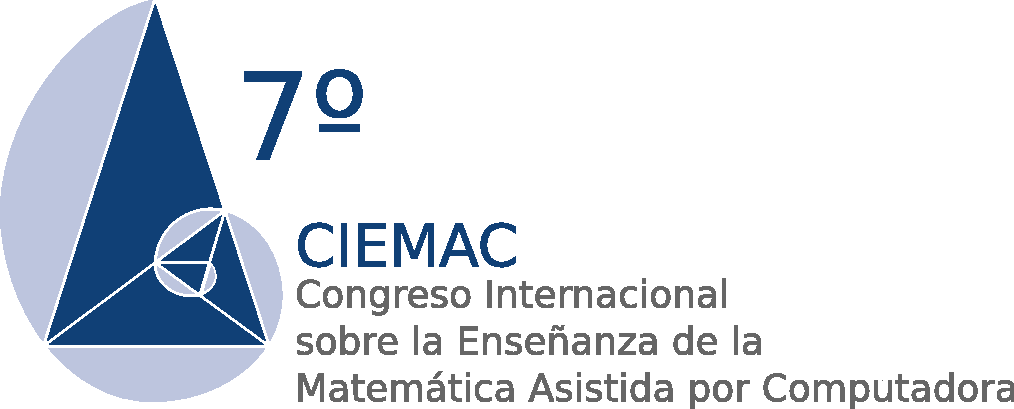
\includegraphics[scale=0.5]{LogoCIEMAC}}}

\AddToBackground{6}{%  Background of a small page
  \put(0,0){\textcolor{Cyan!50}{\rule{\paperwidth}{\paperheight}}}} %YellowOrange

%\AddToBackground{6}{%  Background of a small page
 % \put(10,450){
\includegraphics[scale=1]{LogoTEC}}}

\AddToBackground*{2}{% Background of a large page
  \put(\LenToUnit{.5\paperwidth},\LenToUnit{.5\paperheight}){%
    \makebox(0,0)[c]{%
      \resizebox{.9\paperwidth}{!}{\rotatebox{35.26}{%
        \textsf{\textbf{\textcolor{LIGHTGRAY}{CIEMAC}}}}}}}}
        
\AddToBackground*{1}{% Background of a large page
  \put(0,\LenToUnit{.5\paperheight}){% \LenToUnit{.5\paperwidth}
    \makebox(0,0)[c]{%
      \resizebox{.9\paperwidth}{!}{\rotatebox{20}{%
        
\includegraphics[scale=1.5]{IconoCIEMACTransparente}}}}}}
        
\AddToBackground*{2}{% Background of a large page
  \put(130,100){% \LenToUnit{.5\paperwidth}, \LenToUnit{.5\paperheight}
    \makebox(0,0)[c]{%
      \resizebox{.4\paperwidth}{!}{\rotatebox{30}{%
        
\includegraphics[scale=1]{IconoCIEMACTransparente}}}}}}

\begin{document}

\maketitle

\thispagestyle{empty}

\section{Introducción} 

El Instituto Tecnológico de Costa Rica en respuesta a su compromiso con el desarrollo del país y con su vocación constante de apoyo integral con la educación costarricense tiene el agrado de invitar a profesores y profesoras de matemática de educación media y a maestros y maestras de primaria al $7^\circ$ Congreso Internacional sobre Enseñanza de la Matemática Asistida por Computadora.

Este congreso está orientado a ofrecer a los educadores y educadoras del país tres días de reflexión y capacitación sobre temas relacionados con la matemática y su enseñanza.

La actividad es organizada por la Escuela de Matemática del Instituto Tenológico de Costa Rica.

\newpage

\section{Ejes Temáticos}

El trabajo académico se centrará en los siguientes ejes temáticos:

\begin{itemize}
\item Área de Software para Educación.

\item Área de Desarrollo del Razonamiento.

\item Área de evaluación de software.
\end{itemize}

Se desarrollará fundamentalmente a través de conferencias y talleres de trabajo.


\section{Expositores}

El congreso contará con diversos expositores tanto nacionales como extranjeros, entre los más destacados están:

\begin{itemize}
\item Ricardo Nemirovsky (Estados Unidos)

\item Edison DeFaria (Costa Rica)

\item Norma Noguera (Estados Unidos)

\item José Luis Lupiañez (España)

\item Mario Marín (Costa Rica)

\item Feliú Sagols (México)

\item Victor Palencia (México)

\item Norma Goris (México)

\item Teresa Carrillo (México)
\end{itemize}

\newpage

\section{Recepción de trabajos}

Las modalidades para los trabajos son:

\begin{itemize}
\item Talleres.

\item Cursos cortos

\item Conferencias
\end{itemize}

Le invitamos a enviar sus propuestas al correo \url{aborbon@itcr.ac.cr}, pueden ser talleres de 2, 4 o 6 horas ya sean sobre software o en evaluación  y diseño de actividades curriculares, ponencias que demuestren resultados de investigaciones o reportes de experiencias exitosas en el uso de tecnología en los procesos de enseñanza aprendizaje de la  matemática, éstas  tienen una duración  30 minutos o bien de una hora si el proponente lo justifica. 

Además se desarrollarán otras actividades tendientes a fomentar en los docentes el interés por utilizar software educativo en matemática y en general para ayudarles a crecer profesionalmente mediante la actualización en temas de relevancia como resolución de problemas y uso de software en educación. 

\textcolor{Blue}{La fecha límite para el envío de propuestas es el 15  de septiembre del 2011.}

\section{Cronograma propuesto}

\begin{center}
\rowcolors{1}{gray!5}{gray!20}
\begin{tabular}{| >{\centering\arraybackslash}m{3.3cm} | >{\centering\arraybackslash}m{3.8cm} | >{\centering\arraybackslash}m{3.8cm} | >{\centering\arraybackslash}m{3.8cm} |} \hline %{|p{3.3cm}|p{3.8cm}|p{3.8cm}|p{3.8cm}|} \hline
\rowcolor{LightBlue2} {\bf Hora} & {\bf Miércoles 16} & {\bf Jueves 17} & {\bf Viernes 18}  \\ \hline 
 8:00 am a 9:00 am &  Inscripción, inauguración y desayuno & Conferencia plenaria & Conferencia plenaria \\ \hline 
9:00 am a 10:00 am & Conferencia inaugural & Conferencia plenaria & Conferencia plenaria \\ \hline 
10:00 am a 10:30 am & \multicolumn{3}{|c|}{Refrigerio} \\ \hline 
10:30 am a 12:20 pm & Talleres y ponencias & Talleres y ponencias & Cierre y entrega de certificados \\ \hline 
12:30 pm a 1:30 pm & \multicolumn{3}{|c|}{Almuerzo} \\ \hline 
1:30 pm a 3:00 pm & Talleres y ponencias & Talleres y ponencias &  \\ \hline 
3:00 pm a 3:30 pm & \multicolumn{2}{|c|}{Refrigerio} &  \\ \hline 
3:30 pm a 5:00 pm & Talleres y ponencias & Talleres y ponencias &  \\ \hline 
5:00 pm a 6:00 pm & Actividades de integración & Actividades de integración &  \\ \hline 
\end{tabular}
\end{center}

\newpage

\section{Inscripción y costos}

\begin{center}
\rowcolors{1}{gray!5}{gray!20}
\begin{tabular}{|p{2.6cm}|p{1.7cm}|p{1.7cm}|} \hline
\rowcolor{LightBlue2} {\bf Tipo de participación} & {\bf Inscripción temprana} & {\bf Inscripción general}  \\ %\savehline 
Ponente nacional &  C \hspace*{-4.1mm} \textbar \hspace*{-1.6mm} \textbar 10 000 & C \hspace*{-4.1mm} \textbar \hspace*{-1.6mm} \textbar 25 000 \\ %\savehline 
Ponente extranjero & \$50 & \$60 \\ %\savehline 
Estudiante nacional & C \hspace*{-4.1mm} \textbar \hspace*{-1.6mm} \textbar 12 000 & C \hspace*{-4.1mm} \textbar \hspace*{-1.6mm} \textbar17 000 \\ %\savehline 
Estudiante extranjero & \$60 & \$70 \\ %\savehline 
Participante nacional & C \hspace*{-4.1mm} \textbar \hspace*{-1.6mm} \textbar 20 000 & C \hspace*{-4.1mm} \textbar \hspace*{-1.6mm} \textbar 25 000 \\ %\savehline 
Participante extranjero & \$75 & \$100 \\ \hline 
\end{tabular}
\end{center}

\textcolor{blue}{Observaciones:}

\begin{itemize}
\item Los precios de ponente son para aquellos expositores que desean participar en todo el evento y recibir título de participación.

\item La cuota de inscripción incluye: 5 refrigerios (mañana y tarde), bolso del evento, CD de memorias del evento, título de participación, gafete, programa de actividades, calendario y derecho a asistencia a las actividades incluidas en el programa.
\end{itemize}

\newpage

\section{Comité organizador}

M.Sc. Mario Marín Sánchez, ITCR (coordinador)

M.Sc. Cristhian Páez Páez, ITCR

M.Sc. Alexander Borbón Alpízar, ITCR

M.Sc. Jorge Monge Fallas, ITCR

M.Sc. Cindy Calderón, ITCR

Lic. Rebeca Solís Ortega


\subsection{Comité científico}

M.Sc. Alexander Borbón Alpízar, ITCR (coordinador)

M.Sc. Alcides Astorga Morales, ITCR

Phd. Evelyn Agüero Calvo, ITCR

Lic. Manuel Murillo Tsijli, ITCR

M.Sc. Jorge Monge Fallas, ITCR

\newpage



\section{\vfill Contacto}

Si desea recibir información adicional sobre el congreso o tiene alguna duda del evento, por favor escribir a \url{ciemac@itcr.ac.cr} o a Mario Marín a \url{mmarin@itcr.ac.cr}

Escuela de Matemática

Instituto Tecnológico de Costa Rica

Cartago, Costa Rica

Teléfono: (506)2552-5333 / (506) 2550-2225, Fax: (506) 2550-2493

Apartado Postal: 159-7050 Cartago, Costa Rica

\vspace{1cm}

\begin{center}

\includegraphics[scale=1]{LogoTEC}
\end{center}

\end{document}